% Lit review
% Theory
% Hypotheses
% Data source
% Measurments
% Methods
% Results
% Conclusion
% Limitations/Future

% Previous research:

% - Focus on one field
% - Focus on qualitative

\documentclass[xcolor=dvipsnames]{beamer}

\usepackage{tikz}
\usetikzlibrary{quotes}

\usepackage{multicol}
\usepackage{subcaption}
\usepackage{natbib}
\usepackage{hyperref}
\hypersetup{
    colorlinks=true,
    linkcolor=UniBlue,
    urlcolor=UniBlue,
    citecolor=UniBlue,
}
\usepackage[font=scriptsize]{caption}

\usepackage{changepage}
\usepackage{amsmath,bm}

\beamertemplatenavigationsymbolsempty

\definecolor{UniBlue}{RGB}{83,121,170}
\setbeamercolor{title}{fg=UniBlue}
\setbeamercolor{frametitle}{fg=UniBlue}
\setbeamercolor{structure}{fg=UniBlue}

\title{The Structure of Scientific Fields}
\author{Vladimir Borel}
\institute{University of California, Riverside}
\date{\today}
% \date{}


\newcommand{\insertfigs}[2]{
    \begin{figure}[H]
        \caption{#1}
        \label{fig:#2}
        \foreach \name in \fields {
            \begin{subfigure}[p]{0.15\textheight}
                \centering
                \resizebox{0.8\textwidth}{!}{%
                    \includegraphics[width=\textwidth]{figures/#2/\name}
                }
                \caption{\name}
            \end{subfigure}\quad
        }
    \end{figure}
}

\newcommand{\insertfig}[2]{
    \begin{figure}[H]
        \caption{#1}
        \label{fig:#2}
        \includegraphics[width=\textwidth]{figures/#2}
    \end{figure}
}

\newcommand{\inserttable}[2]{
    \newgeometry{margin=2cm}
    \begin{landscape}
    \begin{table}[H]
        \caption{#1}
        \label{table:#2}
        \resizebox{\columnwidth}{!}{
            \input{tables/#2}
        }
    \end{table}
    \end{landscape}
    \restoregeometry
}

\newcommand{\tableref}[1]{
    \begin{center} 
        \textbf{[Table \ref{table:#1} about here]}
    \end{center}
}

\newcommand{\figref}[1]{
    \begin{center} 
        \textbf{[Fogure \ref{fig:#1} about here]}
    \end{center}
}

\newcommand*{\fields}{
    Artificial intelligence,
    Economics,
    Ethnic \string& cultural studies,
    Gender studies,
    Genetics \string& genomics,
    Geometry,
    Geophysics,
    Human resources \string& organizations,
    Immunology,
    International business,
    Language \string& linguistics,
    Material engineering,
    Neurology,
    Political science,
    Probability \string& statistics,
    Sociology
}

\newcommand{\insertfigsslides}[2]{
    \begin{adjustwidth}{-2em}{-2em}
        \begin{figure}[hbtp]
            % \caption{#1}
            \label{fig:#2}
            \foreach \name in \fields {
                \begin{subfigure}[p]{0.19\textheight}
                    \centering
                    \resizebox{0.75\textwidth}{!}{%
                        \includegraphics[width=\textwidth]{figures/#2/\name}
                    }
                    \caption{\name}
                \end{subfigure}\quad
            }
        \end{figure}
    \end{adjustwidth}
}

\newcommand{\insertfigslides}[1]{
    \includegraphics[keepaspectratio=true,width=\paperwidth, height=\paperheight]{figures/#1}
}

\newcommand*{\bivariates}{
    Density\_AvgDegree,
    Density\_Triangles,
    Density\_Louvain,
    Density\_Components,
    Density\_AvgClustering,
    Density\_Transitivity,
    Density\_Centralization,
    AvgClustering\_Centralization
}

\newcommand{\insertbivariatesslides}[1]{
    \begin{adjustwidth}{-2em}{-2em}
        \begin{figure}[hbtp]
            % \label{fig:#2}
            \foreach \name in \bivariates {
                \begin{subfigure}[p]{0.25\textheight}
                    \centering
                    \resizebox{0.75\textwidth}{!}{%
                        \includegraphics[width=\textwidth]{figures/all_bivariate/\name}
                    }
                    \caption{\name}
                \end{subfigure}\quad
            }
        \end{figure}
    \end{adjustwidth}
}



\begin{document}

\frame{\titlepage}

\begin{frame}
\frametitle{Introduction}
The debates on the structure and dynamics of science have often been based on abstract ideas rather than 
empirical evidence. However, the recent trend towards digitalization of peer-reviewed scientific articles 
has made it possible to test these theories using empirical data. This provides a valuable opportunity to 
advance our understanding of the structure and dynamics of science.

These theories ask a range of questions about the nature of science and its relationship to other fields 
of knowledge. Some of the key questions they address include: 
\begin{itemize}
    \item Are there regular patterns in the way that the structure of science changes?
    \item Is science a distinct field of knowledge or is it embedded in larger domains, is the 
    knowledge generated by scientific methods fundamentally different from other types of knowledge?
    \item Are there clear distinctions between science and non-science or between different types of 
    science (e.g. "hard" and "soft" sciences)? 
\end{itemize}

This paper aims to make three types of contributions. The first set of contributions is theoretical 
and involves synthesizing and unifying different conceptions of scientific development in graph-theoretic 
terms. The second set of contributions is empirical and involves deriving and testing hypotheses from the 
literature on scientific development. The third set of contributions is practical and focuses on developing 
a standard analysis pipeline applicable to a wide variety of fields. This is necessary due to the increasing 
difficulty of coordinating research efforts and bridging "academic silos" in the face of the exponentially 
increasing output of technical knowledge and the fact that researchers only have local knowledge about their 
immediate neighbors.

When discussing the structure of a body of knowledge, I am referring to two main aspects: the citation 
structure and the semantic structure. The citation structure refers to the way in which ideas and information 
are connected through references and citations, while the semantic structure refers to the meaning and relationships 
between the concepts and ideas within the body of knowledge. Both of these aspects of structure are important for 
understanding the organization and development of a particular field of knowledge.


\end{frame}

\begin{frame}
\frametitle{Theory}
\only<1>{

	\framesubtitle{Attention Space \citep{collins1994}}

	% To answer this question Collins posits that all fields are subject to the "Law of Small Numbers"

	% Scientific communities compete for the "attention space" (i.e., resources)

	% A sort of carrying capacity which determines the upper limit of the number of subfields

	% Consolidation or restructuring takes place soon after surpassing the carrying capacity

	\begin{itemize}

		\item “Dynamics of the Law of Small Numbers, dividing the attention space among factions […] a struggle for attention” \citep[158-160]{collins1994}

		\item "In any period of creative life, there are typically between three and six [...] lineages or schools" \citep[157]{collins1994}

		\item "\textbf{Law of Small Numbers}, dividing the \textbf{attention space} among factions" \citep[158]{collins1994}

	\end{itemize}

	\vfill

	$\bm{H_{1}}$: When the \textbf{density of subfields} within a field surpasses six, the field is more likely to experience a tendency towards \textbf{consolidation}.

}

\only<2>{

	\framesubtitle{Moving Frontier \citep{collins1994}}

	% Collins distinguishes between "high-consensus rapid-discovery science" and "low-consensus" science

	% He posits that these "high-consensus rapid-discovery" science have "fast moving research front"

	% "Fast moving research front" as refers to the fact that disagreements are confined to the research frontier

	\begin{itemize}

		\item "High-consensus rapid-discovery science" \citep[157]{collins1994}

		\item \textbf{"Fast moving research front"} \citep[158]{collins1994}

		\item "\textbf{Ready made} science" v. "Science \textbf{in the making}" \citep{latour1988}

	\end{itemize}

	\vfill

	$\bm{H_{1}}$: \textbf{"Hard" sciences} have a \textbf{faster moving "research front"} than "soft" sciences.

}

\only<3>{
	
	\framesubtitle{Research Technology \citep{collins1994}}

	% So how does he explain the difference between "high-consensus rapid-discovery" science and "low-consensus" science?

	% Well, ite relies on the institutionalization of practices

	% Specifically: "routinized" research practices

	% Groups form around a technology which produces consistent & reliable outputs

	% So, for Collins, what distinguises "high-consensus rapid-discovery" science, is not "empiricism", "measurement precision", "formalization", or the "experimental method", but a "genealogy of technologies" producing reliable results.

	\begin{itemize}

		\item What sets appart "\textbf{high-consensus rapid-discovery}" from "\textbf{low-consensus non-rapid-discovery}" science? \citep[158]{collins1994}

		\item Not "empiricism", "measurement precision", "formalization", or the "experimental method" \citep[158]{collins1994}

		\item "\textbf{Genealogy of research technology}" producing reliable observation \citep[158]{collins1994}

	\end{itemize}

	\vfill

	$\bm{H_{2a}}$: A \textbf{change in "research technologies"} should change the structure of the \textbf{"hard" sciences}, while these changes should be absent altogether in "soft" sciences.
}

\only<4>{

	\framesubtitle{Social conditions \citep{collins1994}}

	% 

	“\textbf{Political and economic conditions} change [the] \textbf{material bases} supporting intellectual life, [they] provoke [the] \textbf{realignment of factions”} \citep[165]{collins2000}
	
	\vfill

	$\bm{H_{2b}}$: A \textbf{change in social or political conditions} should change the structure of the \textbf{"soft" sciences}, while these changes should be absent altogether in "hard" sciences.

}

\only<5>{

	\framesubtitle{Scientific Revolutions \citep{kuhn2012}}

	\begin{itemize}

		% In Kuhn's model, sciences go through periods of relative stability (i.e., "normal" or "paradigmatic" science) 

		% Anomalies accumulate.

		% Anomalies are observation that do not fit the current models

		% As anomalies accumulate

		% New paradigms emerge and compete

		% Scientific revolution ends when consensus is reached

		% Compares them to political revolutions
		% One institution must die for the next one to be born

		% Basis of science is community consensus (e.g., textbook, curriculums, etc.)


		\item “Political revolutions aim to change political institutions in ways that those institutions themselves prohibit […] necessitates the partial relinquishment of one set of institutions in favor of another […] Initially it is crisis […] that attenuates the role of political institutions […] and the role of paradigms” \citep[93]{kuhn2012}

		\item "Recurrent debates about whether one or another of the contemporary social sciences is really a science [...] will cease to be a source of concern not when a definition is found, but when the groups that now doubt their own status achieve consensus about their past and present accomplishments” \citep[161]{kuhn2012}

	\end{itemize}
	
	\vfill

	$\bm{H_{4}}$: Disciplines generally exhibit \textbf{stability}, with occasional episodes of significant \textbf{changes}.

}

\only<6>{

	\framesubtitle{Self-Similarity \citep{abbott2001}}

	\begin{itemize}

		\item “Fractal pattern of division and convergence” \citep{abbott2001}

		\item “The quantitative – qualitative distinction repeats itself at each more detailed level even as the difference between positions narrows” \citep{harty2004}

	\end{itemize}

	\vfill
	$\bm{H_{6}}$: Within the field, subfields arise, exhibiting a replication of the core structure and retaining distinct features of the broader discipline.

}


% % of articles each year that use a term

% % Communities around technologies & ideas 
% % Reliable expected results





% \only<1>{
% 	\framesubtitle{Science as High Consensus, Rapid Discovery Science}
% 	\begin{itemize}

% 		\item "\textbf{Consensus} is not the prevailing pattern [...] \textbf{disagreement} is the norm" \citep[157]{collins1994}

% 		\item What sets appart "\textbf{high-consensus rapid-discovery}" from "\textbf{low-consensus non-rapid-discovery}" science? \citep[158]{collins1994}

% 		\item Not "empiricism", "measurement precision", "formalization", or the "experimental method" \citep[158]{collins1994}

% 		\item "\textbf{Genealogy of research technology}" producing reliable observation \citep[158]{collins1994}

% 		\item Fast moving research front 158

% 		\item "\textbf{Ready made} science" v. "Science \textbf{in the making}" \citep{latour1988}

% 		\item "intensive research goes for the fundamental laws, extensive research goes for the explanation of phenomena in terms of known fundamental laws" \citep[393]{anderson1972}

% 	\end{itemize}
% }

% \only<2>{
% 	\framesubtitle{Science as Attention Space}
% 	\begin{itemize}
% 		\item "In any period of creative life, there are typically \textbf{between three and six [...] lineages or schools}" \citep[157]{collins1994}.
% 		\item "\textbf{Law of Small Numbers}, dividing the \textbf{attention space} among factions" \citep[158]{collins1994}
% 	\end{itemize}
% }

% \only<3>{
% 	\framesubtitle{Science as Revolutionary}
% 	\begin{itemize}
% 		\item "Intellectual \textbf{crisis}, followed by restructuring [...] reduces the number of lineages to the normal ceiling" \citep[157]{collins1994}.
% 		\item During "\textbf{normal science}" "\textbf{anomalies accumulate}"  leading to a phase of "\textbf{revolutionary science}" and a "\textbf{paradigm change}" \citep{kuhn2012}
% 	\end{itemize}
% }

% \only<4>{
% 	\framesubtitle{Science as Technology}
% 	\begin{itemize}
% 		\item "Intellectual community consists in networks that pass \textbf{ideas} [...], research \textbf{technologies} comprise a parallel set of networks" \citep[164]{collins1994}
% 		\item "Human and machine networks develop symbiotically" \citep[164]{collins1994}
% 		\item "\textbf{Human} and \textbf{non-human} network actors" \citep{latour1988}
% 	\end{itemize}
% }

% \only<5>{
% 	\framesubtitle{Science as Institution}
% 	\begin{itemize}
% 		\item "Research equipment, once \textbf{routinized}, may be exported from the laboratory" \citep[165]{collins1994}
% 		\item "Technological \textbf{routine}" \citep[165]{collins1994}
% 		\item “Political \textbf{revolutions} aim to change political institutions in ways that those institutions themselves prohibit […] necessitates the partial \textbf{relinquishment of one set of institutions} in favor of another” \citep[93]{kuhn2012}
% 		\item “Cluster’s social [structural] change is accompanied by intellectual [content] changes” \citep[22]{mullins1973}
% 	\end{itemize}
% }

% \only<6> {
% 	\framesubtitle{Science as Fractal}

% 	\citep{abbott2001}

% 	% \noindent\includegraphics[width=\linewidth]{figures/fractal_distinctions}

% 	\begin{figure}[H]
	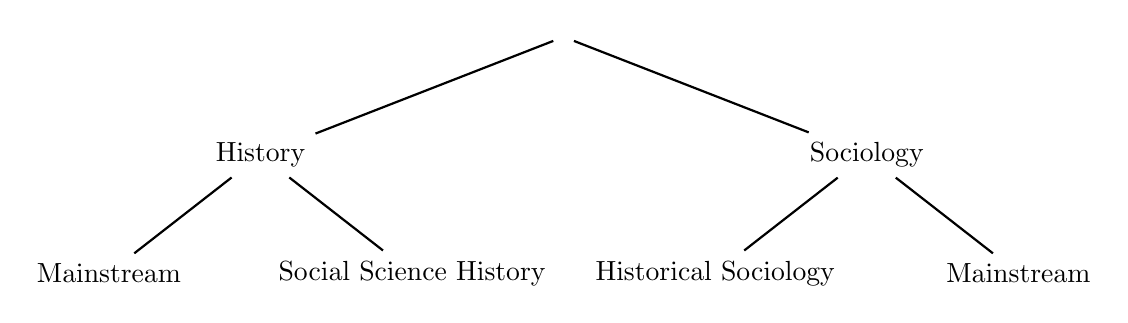
\begin{tikzpicture}[thick,level/.style={sibling distance=77mm/#1}]
	\node [] (r) {}
	  child {
	    node [] (a) {History}
	    child {
	      node [] {Mainstream}
	    }
	    child {
	      node [] {Social Science History}
	    }
	  }
	  child {
	    node [] {Sociology}
	    child {
	      node [] {Historical Sociology}
	    }
	    child {
	      node [] {Mainstream}
	    }
	  };
	\end{tikzpicture}
	\caption{Fractal Distinctions} 
	\label{fig:fractal_distinctions}
\end{figure}

% 	% \begin{figure}
% 	% \begin{tikzpicture}[thick,level/.style={sibling distance=100mm}]
% 	% \node [] (r) {}
% 	%   child {
% 	%     node [] (a) {History}
% 	%     child {
% 	%       node [] {Mainstream}
% 	%     }
% 	%     child {
% 	%       node [] {Social Science History}
% 	%     }
% 	%   }
% 	%   child {
% 	%     node [] {Sociology}
% 	%     child {
% 	%       node [] {Historical Sociology}
% 	%     }
% 	%     child {
% 	%       node [] {Mainstream}
% 	%     }
% 	%   };
% 	% \end{tikzpicture}
% 	% \caption{Fractal Distinctions} 
% 	% \label{fig:fractal_distinctions}
% 	% \end{figure}
% }












\end{frame}

% \begin{frame}
% \frametitle{DAG}
% \begin{figure}[H]
    \centering
    % \begin{subfigure}[t]{0.1\textwidth}
    %     \centering
    %     \begin{tikzpicture}[node distance=2cm, thick, main/.style = {draw, circle}]
    %         \node[draw=none] (1) [below left of=2] {};
    %         \node[draw=none] (2) [above left of=2] {};
    %         \path[->,draw,thick]
    %         (1) edge node[pos=0.5, left] {$t$} (2);
    %     \end{tikzpicture}
    % \end{subfigure}
    \begin{subfigure}[t]{0.2\textwidth}
        \centering
        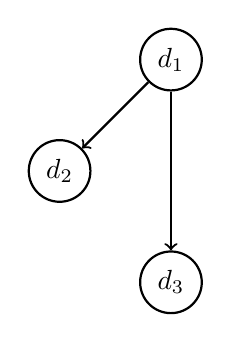
\begin{tikzpicture}[node distance=2cm, thick, main/.style = {draw, circle}]
            \node[main] (1) [] {$d_1$};
            \node[main] (2) [below left of=1] {$d_2$};
            \node[main] (3) [below right of=2] {$d_3$};
            \path[->,draw,thick]
            (1) edge node[] {} (2)
            (1) edge node[] {} (3);
        \end{tikzpicture}
    \end{subfigure}
    ~
    \begin{subfigure}[t]{0.2\textwidth}
        \centering
        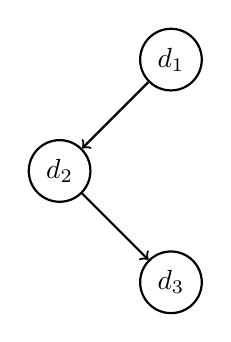
\begin{tikzpicture}[node distance=2cm, thick, main/.style = {draw, circle}]
            \node[main] (1) [] {$d_1$};
            \node[main] (2) [below left of=1] {$d_2$};
            \node[main] (3) [below right of=2] {$d_3$};
            \path[->,draw,thick]
            (1) edge node[] {} (2)
            (2) edge node[] {} (3);
        \end{tikzpicture}
    \end{subfigure}
    ~
    \begin{subfigure}[t]{0.2\textwidth}
        \centering
        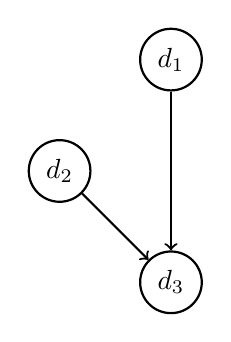
\begin{tikzpicture}[node distance=2cm, thick, main/.style = {draw, circle}]
            \node[main] (1) [] {$d_1$};
            \node[main] (2) [below left of=1] {$d_2$};
            \node[main] (3) [below right of=2] {$d_3$};
            \path[->,draw,thick]
            (1) edge node[] {} (3)
            (2) edge node[] {} (3);
        \end{tikzpicture}
    \end{subfigure}
    ~
    \begin{subfigure}[t]{0.2\textwidth}
        \centering
        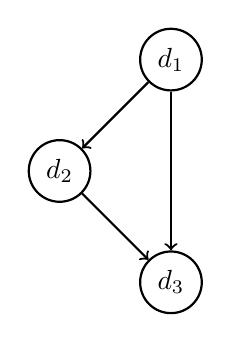
\begin{tikzpicture}[node distance=2cm, thick, main/.style = {draw, circle}]
            \node[main] (1) [] {$d_1$};
            \node[main] (2) [below left of=1] {$d_2$};
            \node[main] (3) [below right of=2] {$d_3$};
            \path[->,draw,thick]
            (1) edge node[] {} (2)
            (2) edge node[] {} (3)
            (1) edge node[] {} (3);
        \end{tikzpicture}
     \end{subfigure}
     \caption{DAG}
\end{figure}
% \end{frame}

% \begin{frame}
% \frametitle{Networks}
% \only<1>{

\begin{itemize}
    \item Citation: Directed Acyclic
    \item Co-Citation: Undirected weighted
    \item Co-Occurrence: Unidrected weighted
\end{itemize}

\begin{figure}
    \centering
    \begin{minipage}[b]{0.25\textwidth}\centering
        \begin{figure}[H]
    \centering
    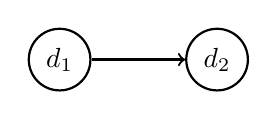
\begin{tikzpicture}[node distance=2cm, thick, main/.style = {draw, circle}]
        \node[main] (1) [] {$d_1$};
        \node[main] (2) [right of=1] {$d_2$};
        \draw[->] (1) -- (2);
    \end{tikzpicture}
    \caption{Citation} \label{fig:citation}
\end{figure}
    \end{minipage}\hfill
    \begin{minipage}[b]{0.33\textwidth}\centering
        \begin{figure}[H]
    \centering
    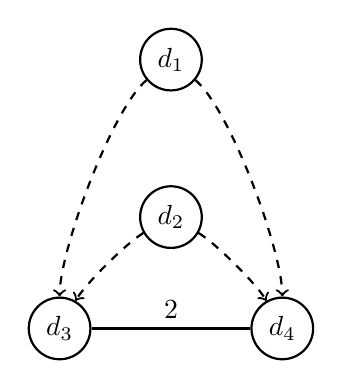
\begin{tikzpicture}[node distance=2cm, thick, main/.style = {draw, circle}]
        \node[main] (1) [] {$d_1$};
        \node[main] (2) [below of=1] {$d_2$};
        \node[main] (3) [below left of=2] {$d_3$};
        \node[main] (4) [below right of=2] {$d_4$};
        \draw[->] (1) to [out=220, in=90, looseness=0.5] (3) [dashed] node {};
        \draw[->] (1) to [out=320, in=90, looseness=0.5] (4) [dashed] node {};
        \draw[->] (2) to [out=210, in=60, looseness=0.5] (3) [dashed] node {};
        \draw[->] (2) to [out=330, in=120, looseness=0.5] (4) [dashed] node {};
        \draw[] (3) -- node[midway, above] {2} (4);
    \end{tikzpicture}
    \caption{Co-Citation} \label{fig:co_citation}
\end{figure}
    \end{minipage}\hfill
    \begin{minipage}[b]{0.33\textwidth}\centering
        \begin{figure}[H]
    \centering
    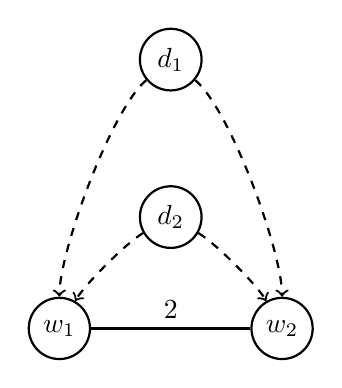
\begin{tikzpicture}[node distance=2cm, thick, main/.style = {draw, circle}]
        \node[main] (1) [] {$d_1$};
        \node[main] (2) [below of=1] {$d_2$};
        \node[main] (3) [below left of=2] {$w_1$};
        \node[main] (4) [below right of=2] {$w_2$};
        \draw[->] (1) to [out=220, in=90, looseness=0.5] (3) [dashed] node {};
        \draw[->] (1) to [out=320, in=90, looseness=0.5] (4) [dashed] node {};
        \draw[->] (2) to [out=210, in=60, looseness=0.5] (3) [dashed] node {};
        \draw[->] (2) to [out=330, in=120, looseness=0.5] (4) [dashed] node {};
        \draw[] (3) -- node[midway, above] {2} (4);
    \end{tikzpicture}
    \caption{Co-Occurrence} \label{fig:co_occurrence}
\end{figure}

    \end{minipage}
\end{figure}

}

% \only<2>{

%     \begin{table}[H]
%         % \caption{$G = (N, E)$}
%         \resizebox{\linewidth}{!}{
%             \begin{tabular}{lrrrrrr}
\toprule
                                & \multicolumn{2}{l}{Citation} & \multicolumn{2}{l}{Co-Citation} & \multicolumn{2}{l}{Co-Occurrence} \\
                          Field &    Nodes &  Edges &       Nodes &  Edges &         Nodes &   Edges \\
\midrule
                 Gender Studies &     2224 &   4332 &         439 &    810 &         18375 & 2362724 \\
                       Geometry &     2314 &   2995 &         298 &    388 &         11881 & 1119429 \\
                     Geophysics &    38952 & 162177 &       16305 &  82952 &         21341 & 3709723 \\
                      Economics &     7147 &  55537 &        4278 &  53161 &         12780 & 1347658 \\
         Language \& Linguistics &     3128 &  13572 &        1270 &   7819 &         14771 & 1955723 \\
       Probability \& Statistics &     5496 &  19273 &        1805 &   8151 &         15127 & 2272474 \\
           Material Engineering &    39045 & 253189 &       19577 & 213117 &         20958 & 3361647 \\
        Artificial Intelligence &     5475 &  21705 &        1897 &   9012 &         15040 & 2598151 \\
                      Sociology &     4083 &  25676 &        2327 &  21230 &         16822 & 2381323 \\
         International Business &     5254 &  36786 &        2667 &  39483 &         13395 & 1955815 \\
              Political Science &     5305 &  26335 &        2442 &  13314 &         16461 & 2126471 \\
            Genetics \& Genomics &    26776 & 109991 &        9323 &  55121 &         22220 & 3447289 \\
                     Immunology &    27301 & 195148 &       12636 & 190468 &         22126 & 3990841 \\
Human Resources \& Organizations &     5848 &  34965 &        3063 &  24554 &         14355 & 2170039 \\
      Ethnic \& Cultural Studies &     2105 &   4041 &         310 &    506 &         15986 & 2037714 \\
                      Neurology &    32881 & 282230 &       18589 & 270528 &         20501 & 3662226 \\
\bottomrule
\end{tabular}

%         }
%     \end{table}

% }
% \end{frame}

% \begin{frame}
% \frametitle{Data}
% Having established the possibility of linking citation networks and concept networks as clusters at various levels of analysis, I will now delve into a discussion of the data used to identify the structure and dynamics of scientific communities. The analysis of this data will enable me to evaluate the accuracy of the various theories of scientific development discussed earlier and to provide a realistic account of the fields analyzed, given that the data is reliable and sufficient.

\subsubsection{Sample}

There are two main ways of bounding citation networks. The first involves sampling based on journals \citep{beam2014, moody2006}, while the second involves sampling based on a topical search \citep{borrett2014,callon2005,chavalarias2013}. In this study, I used the former method, selecting articles that were published in one of the 5 peer-reviewed journals with the highest impact factor.

The main advantage of sampling based on journals is that it will allow us to focus on articles published in high-quality, reputable journals. This can help ensure that the data used in the study is of a high quality and is representative of the broader field of research. Additionally, journal-based sampling can make it easier to compare the results of different studies, as it provides a common frame of reference.

Bradford's law \citep{bradford1985, hjorland2005} is a principle that describes the relationship between the number of scientific journals in a particular field and the number of citations that articles in those journals receive. It states that a small number of highly-cited journals tend to publish a disproportionate number of highly-cited articles, while a large number of low-cited journals tend to publish a disproportionate 
number of low-cited articles.

This law can be used to support the choice of only selecting a small number of journals in each scientific field under study. Focusing on a select group of highly-cited journals, can increase the chances of finding and reading the most influential and highly-cited articles in that field. It's worth noting that Bradford's law is not a hard and fast rule, and there may be cases where it is necessary or beneficial to review a larger number of journals in a particular field. However, as a general principle, Bradford's law can be a useful guide when selecting journals for review.

The data used in this study consists of peer-reviewed scientific articles collected by Clarivate Web of Science. These data include each document's citation information, as well as its title, 
abstract, key words, and publication date.

\subsubsection{Fields}

The fields being analyzed include Artificial Intelligence, Astronomy \& Astrophysics, Economics, Ethnic \& Cultural Studies, Gender Studies, Genetics \& Genomics, Geometry, Geophysics, Human Resources \& Organizations, Immunology, International Business, Language \& Linguistics, Law, Material Engineering, Neurology, Political Science, Probability \& Statistics, Sociology, Biochemistry. A complete list of the journals for each of the fields can be found in the Appendix.

These fields were selected for analysis because they represent a diverse range of disciplines, including both hard sciences, as well as soft sciences. This diversity allows for a comprehensive examination of how scientific communities function across different areas of study. Additionally, these fields are dynamic and rapidly advancing, providing a rich source of data for analysis and making them well suited for studying the structure and dynamics of scientific communities. 

Furthermore, these fields were selected because they enable not only the analysis of individual fields but also the use of a comparative framework. Comparing and contrasting the structures and dynamics of scientific communities across different fields allows for a deeper understanding of the similarities and differences among them, and the opportunity to identify common as well as idiosyncratic patterns and trends that may be relevant to theories of scientific development.

\subsubsection{Tools}

Python was used for the analysis \citep{rossum2010}, and several libraries were particularly noteworthy, including Networkx \citep{hagberg2008}, PyMC \citep{wiecki2023} and Polars \citep{vink2023}, among many others.

% \end{frame}

% \begin{frame}
% \frametitle{Citation Networks}
% \insertfigsslides{Citation}{citation_graphs}
% \end{frame}

% \begin{frame}
% \frametitle{E.g., Citation Network}
% \insertfigslides{citation_graphs/Geophysics}
% \end{frame}

% \begin{frame}
% \frametitle{Co-Citation Networks}
% \insertfigsslides{Co-Citation}{co_citation_graphs}
% \end{frame}

% \begin{frame}
% \frametitle{E.g., Co-Citation Network}
% \insertfigslides{co_citation_graphs/Sociology}
% \end{frame}

% \begin{frame}
% \frametitle{Co-Occurrence Networks}
% \insertfigsslides{Co-Occurrence}{co_occurrence_graphs}
% \end{frame}

% \begin{frame}
% \frametitle{E.g., Co-Occurrence Network}
% \insertfigslides{co_occurrence_graphs/Sociology}
% \end{frame}

% \begin{frame}
% \frametitle{E.g., Co-Occurrence Network}
% \insertfigslides{co_occurrence_graphs/Geophysics}
% \end{frame}

% \begin{frame}[allowframebreaks]
% \frametitle{ERGM}
% Exponential Random Graph Models are used to model and test different hypotheses about the 
structural features of social networks. This approach enables us to investigate the different 
local and global properties of a network and establish their importance in explaining its 
formation. By testing for various network properties, such as triangles or the average shortest 
path between nodes, we can determine whether these properties played a significant role in the 
network's formation.

According to the Hammersly and Clifford Theorem (1971), any network model can be expressed in the 
exponential family with counts of graph statistics. The probability of observing a particular graph 
$y$ on $n$ nodes out of the set of all possible graphs on $n$ nodes, $Y$, denoted as $P$, can be 
calculated using a set of network statistics $S$ and corresponding parameters $\theta$.

$$
P_{y,\theta}(Y=y|\theta) = \frac{exp\{\theta^T S(y)\}}{\sum\limits_{y' \in Y} exp\{\theta^T S(y')\}}
$$

The denominator is a normalizing constant that guarantees the distribution adds up to one. 
This constant requires summing over space of possible networks on $n$ nodes. However, the number 
of possible configurations (size of $Y$) grows exponentially with the number of nodes, specifically 
to $2^{(n(n-1)/2)}$ for undirected graphs and $2^{(n(n-1))}$ for directed graphs. Thus, an exact 
computation of this sum is not feasible.

Because of this, it is custommary to use Marcov Chain Monte Carlo method to generate samples. It 
estimate the values of the parameters that maximize the likelihood of the observed network. These 
estimates represent the strength and direction of the effects of various network statistics on the 
likelihood of observing the network.

The above formula can be rewritten in terms of the covariate vector $\theta$:

$$
logit(Y_{ij} | y_{ij}^c) = \theta' \delta(y_{ij})
$$

Where
\begin{itemize}
\item $y_{ij}^c$ is the complement of $y_{ij}$, i.e. all dyads in the network other than $y_{ij}$
\item $y_{ij}^+$ as the same network as $y$ except that $y_{ij} = 1$
\item $y_{ij}^-$ as the same network as $y$ except that $y_{ij} = 0$
\item $\delta(y_{ij})$ is given by $g(y_{ij}^+) - g(y_{ij}^-)$ which measures how the sufficient 
statistic $g(y)$ changes if the $(i, j)$th edge is "toggled" on or off.
\end{itemize}

In sum, for each of the following sufficient statistics a $n \times n$ matrix $s$ is constructed. 
The entry $s_{ij}$ indicates how the presence of the edge between $i$ and $j$ changes the network 
statistic, holding the rest of the network constant.

% \end{frame}

% \begin{frame}
% \frametitle{Measurements}
% 

Following \citet{jiao2017} I define the network measurments and the expected direction of their effect


\subsubsection{Density effect (Edges)}

Density refers to the proportion of connections in a social network relative to the total possible connections.

This is interpreted as the intercept of the model. The entry of the `density` matrix $M_{ij}$ 
indicates how the presence of that edge changes the number of edges in the graph, holding the 
rest of the network constant. It a matrix of ones - with the upper right triangle masked in the 
case of undirected networks.

\subsubsection{Small-World effect (Triangles)}

Social networks tend to exhibit a much higher number of triangles and transitive triads than what 
would be predicted by random graphs with comparable density.

Triangles, which represent a set of three documents or concepts who are mutually connected, are a common feature of social networks and are thought to play an important role in social cohesion and network structure \citep{kossinets2006, newman2018}.

The entry of the triangle matrix $M_{ij}$ indicates how the presence of that edge changes the number of triangles in the graph, holding the rest of the network constant. 

Overall tendency of networks to be composed of local densities (closure). Are the ties randomly distributed of do they form local structures.A graph with a low triangle effect would look homogeneous distribution of substructures is what we would expect from a random graph

Lumps appear (local structures)

\subsubsection{Closure effect (Transitivity)}

A triad is a group of three nodes in a graph. A triad can either be open or closed. An open triad is a group of three nodes that are connected by two edges (Figure \ref{fig:open_triad}), while a closed triad is a group of three nodes that are connected by three edges (Figure \ref{fig:closed_triad}). 

\begin{figure}[H]
    \centering
    \begin{subfigure}[t]{0.4\textwidth}
        \centering
        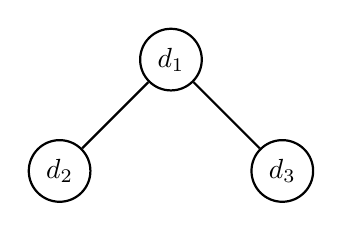
\begin{tikzpicture}[node distance=2cm, thick, main/.style = {draw, circle}]
            \node[main] (1) [] {$d_1$};
            \node[main] (2) [below left of=1] {$d_2$};
            \node[main] (3) [below right of=1] {$d_3$};
            \draw[] (1) to (2);
            \draw[] (1) to (3);
        \end{tikzpicture}
        \caption{Open Triad} 
        \label{fig:open_triad}
     \end{subfigure}
        ~
     \begin{subfigure}[t]{0.4\textwidth}
        \centering
        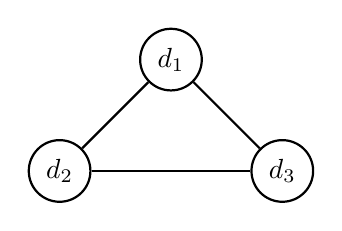
\begin{tikzpicture}[node distance=2cm, thick, main/.style = {draw, circle}]
            \node[main] (1) [] {$d_1$};
            \node[main] (2) [below left of=1] {$d_2$};
            \node[main] (3) [below right of=1] {$d_3$};
            \draw[] (1) to (2);
            \draw[] (1) to (3);
            \draw[] (2) to (3);
        \end{tikzpicture}
        \caption{Closed Triad} 
        \label{fig:closed_triad}
     \end{subfigure}
     \caption{Triads}
\end{figure}

Transitivity is defined as the ratio of the number of closed triads in the graph to the number of open triads in the graph.

$$
T = \frac{3t_c}{t_o}
$$

Where $t_c$ is the number of closed triads and $t_o$ is the number of open triads.


\subsubsection{Clique effect (Cliques)}

Tendecy for there to be parts of the graph where multiple nodes all co-occur more than by random change

If I discuss 
A all other concepts in the clique it belongs to.
highly related to each other distinct topical or functional units within the network

This build on triangles (which are a clique) but captures more information 

It asks whether triangles overlap to form larger structurees rather than just isolated (random) triangles

Densly connected always connected

\subsubsection{Silo effect (Components)}

silos refer to isolated areas of research or knowledge that are not well connected to other areas or fields limit the flow of information and influence within the network
Hyper specialization of field of knowledge
Talk to one another but never talk to nodes outside their primary group

\subsubsection{Popularity effect ($k$-star)}

The popularity effects in most classes were not obvious, which meant the degree (the total number of actors selecting an individual) of individuals in the class networks had little difference.

\begin{figure}[H]
    \centering
    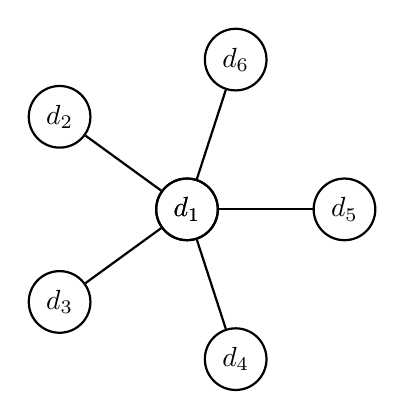
\begin{tikzpicture}[node distance=2cm, thick, main/.style = {draw, circle}]
        \node[main] (1) at (360:0mm) (center) {$d_1$};
        \node[main] (1) [] {$d_1$};
        \foreach \n in {2,...,6}{
            \node[main] at ({\n*360/5}:2cm) (n\n) {$d_\n$};
            \draw (center)--(n\n);
        }
    \end{tikzpicture}
    \caption{Star} \label{fig:k_star}
\end{figure}

What we mean by a strong k star effect
Control for 9 stars in order to determine if 10 star is significant
10 star is a bunch of 9 stars

\subsubsection{Mediating effect (betweenness centrality)}

Nodes with high betweenness centrality in this type of network may represent important bridge terms or pivot terms that connect different topics or themes within the corpus of documents. The betweenness centrality $c_b$ of node $n$ is given by:

$$
c_b(i) = \sum_{j \ne k} \frac{\sigma_{jk}(i)}{\sigma_{jk}}
$$

Where $\sigma_{ij}$ is the total number of shortest paths from node $i$ to node $j$ and $\sigma_{ij}(n)$ is the number of those paths that pass through node $n$. In other words, it is the proportion of all shortest paths between nodes $i$ and $j$ that pass through node $n$. The average betweenness centrality over all nodes of the network is taken as another network statistic. 

Indicates good integration but maybe structural fragility (if central nodes are removed, speperate components)

\subsubsection{Community effect (Louvain)}

The Louvain community detection method consists of two main steps. Initially, each node is assigned to a separate community. Then, for each node, the algorithm attempts 
to optimize the modularity of the network by evaluating the potential gain in modularity achieved by 
moving the node to each of its neighboring communities. If no gain is achieved, the node remains in 
its original community.

In the second step, a new network is constructed where each node represents a community from the 
previous step. The edges between the new nodes are weighted by the sum of the weights of the edges 
between the nodes in the corresponding communities in the original network. The Louvain method is then 
applied to this new network, and the process is repeated until no further improvement in modularity 
can be achieved.

Modularity is a measure of the degree of segregation of a network into communities. It is calculated 
as the difference between the fraction of edges within a given group and the expected fraction of 
edges if they were randomly distributed in the network. The change in modularity $\Delta Q$ achieved 
by moving the node to each of its neighboring communities is measured as

$$
Q = \frac{1}{2m}\sum_{i,j}[A_{ij} - \frac{k_ik_j}{2m}]\delta(c_i,c_j)
$$

where:
\begin{itemize}
    \item $Q$ is the modularity index
    \item $m$ is the total number of edges in the network
    \item $A_{ij}$ is the weight of the edge between nodes $i$ and $j$
    \item $k_i$ and $k_j$ are the degrees of nodes $i$ and $j$, respectively
    \item $c_i$ and $c_j$ are the community assignments of nodes $i$ and $j$
    \item $\delta(c_i,c_j)$ is the Kronecker delta, which is equal to 1 if nodes $i$ and $j$ are in the same community and 0 otherwise.
\end{itemize}

% \subsection{Importance effect (closeness)}

% Nodes with high closeness centrality in these networks may represent important key concepts or core ideas that are central to the understanding of the corpus of documents or, conversly, those that constitute the periphery within the network and are relatively more isolated. On a graph of $n$ nodes, closeness centrality is defined as

% $$
% c_c(i) = \frac{n - 1}{\sum\limits_{i \ne j} d(i, j)}
% $$

% Where $d(i,x)$ is the distance (length of the shortest path) between nodes $i$ and $y$. The average closeness centrality over all nodes of the network is taken as another network statistic. 

% Integration of the field
% Concepts play integrating
% Separated by few or many logical steps

% \subsection{Community centrality (Eigenvector)}

% Eigenvector centrality is a network measure that assigns a score to each node in a network based on the node's connections to other high-scoring nodes. This measure takes into account not only the number of connections a node has, but also the quality or importance of those connections. The average closeness centrality over all nodes of the network is taken as another network statistic.


% \subsection{Concentration effect (Centralization)}

% Measure of the degree of concentration of edges. Centralization is obtained by computing the ratio of the differences between the highest scoring node and all other nodes for both the observed and a star network of the same size.

% $$
% D(G) = \sum_i (max(c) - c_i)
% $$

% where $c_i$ is the centrality $c$ of node $i$ and $max(c)$ is the largest centrality score in graph $G$.  by the maximum theoretical score for a graph with the same number of vertices:

% $$
% C(G) = \frac{D(G)}{D(G_{star})}
% $$


% \subsection{Inequality effect (Gini coefficient)}


% The Gini coefficient in a network can be defined as the ratio between the area between the Lorenz curve and the line of perfect equality ($A$) to the area under the line of perfect equality ($A + B$). The line of perfect equality is a straight line that represents a situation in which all nodes has the same number of edges. The Lorenz curve plots the cumulative proportion of edges against the cumulative proportion of nodes.

% $$
% G = \frac{A}{A + B}
% $$

% As $A$ grows relative to $B$, the fraction tends towards 1, indicating perfect inequality. Conversely, As $B$ grows raltive to $A$, the faction tends towards 0, indicating perfect equality.

% \subsection{Geodesic distance}

% To calculate the average geodesic distance, the shortest path length between every pair of nodes 
% is first computed, and then the average of all these distances is taken. The result is a single value 
% that represents the typical distance between any two nodes in the graph.


% \end{frame}

% \begin{frame}
% \frametitle{Analysis}
% \begin{minipage}[t]{0.4\textwidth}\centering
	\begin{itemize}
		\item Polars \raisebox{-0.3\height}{
\includegraphics[height=0.5cm]{logos/polars}}
		\item Pymc \raisebox{-0.3\height}{
\includegraphics[height=0.5cm]{logos/pymc}}
		\item Seaborn \raisebox{-0.3\height}{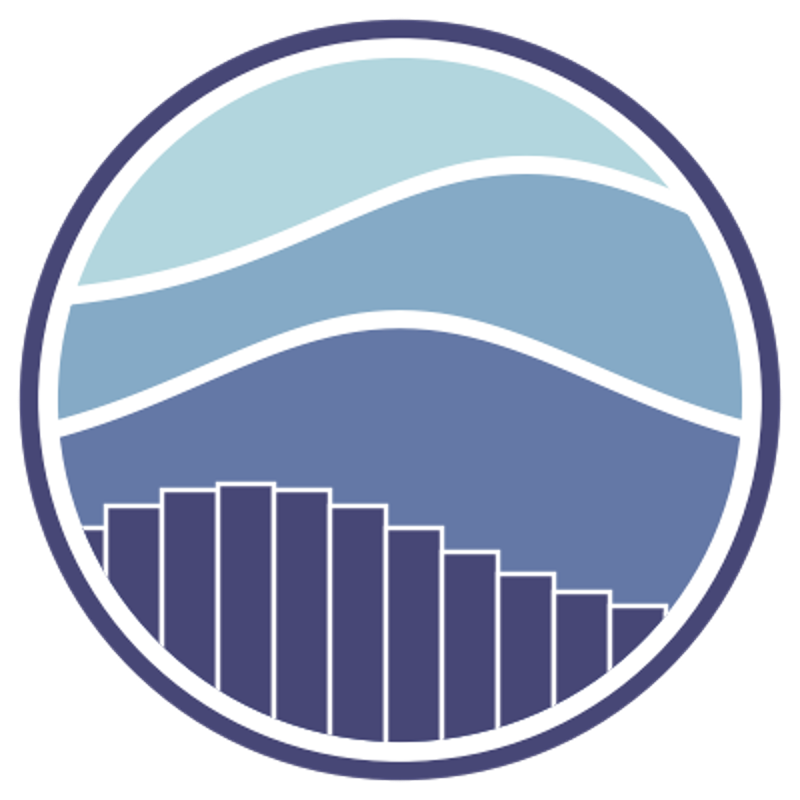
\includegraphics[height=0.5cm]{logos/seaborn}}
		\item Nltk \raisebox{-0.3\height}{
\includegraphics[height=0.5cm]{logos/nltk}}
		\item Numpy \raisebox{-0.3\height}{
\includegraphics[height=0.5cm]{logos/numpy}}
		\item Rust \raisebox{-0.3\height}{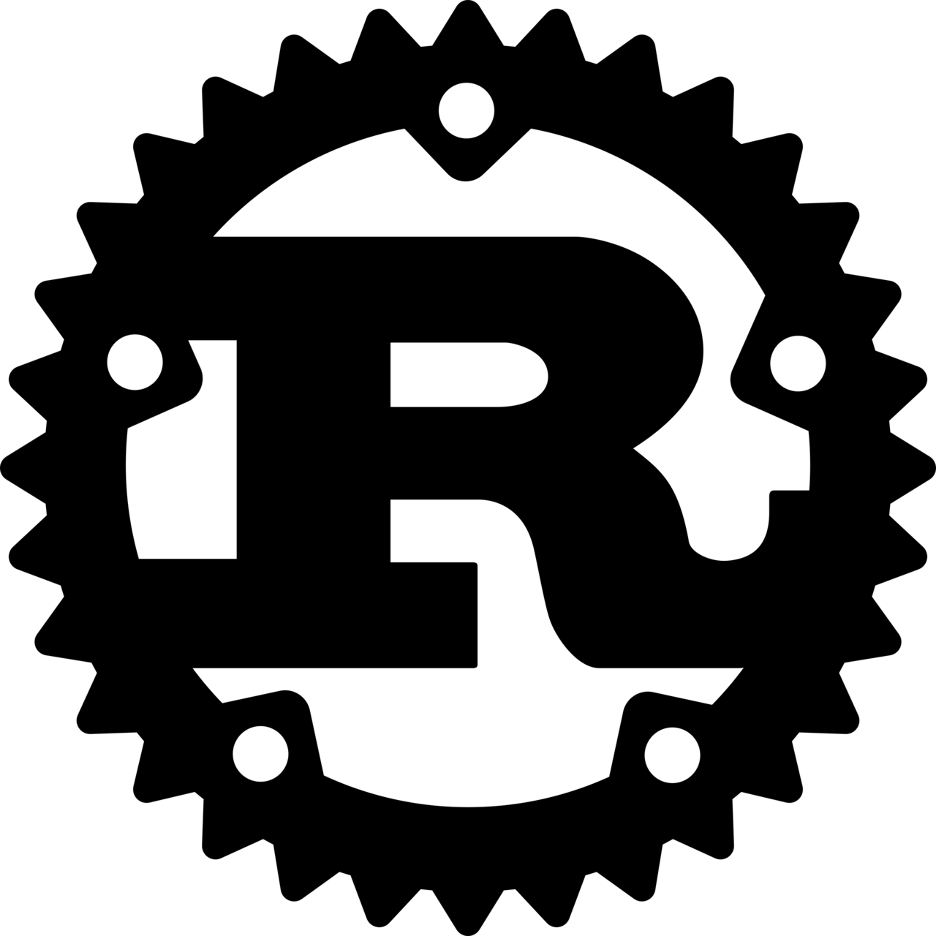
\includegraphics[height=0.5cm]{logos/rust}}
	\end{itemize}
\end{minipage}\hfill
\begin{minipage}[t]{0.4\textwidth}\centering
	\begin{itemize}
		\item Networkx \raisebox{-0.3\height}{
\includegraphics[height=0.5cm]{logos/networkx}}
		\item Matplotlib \raisebox{-0.3\height}{
\includegraphics[height=0.5cm]{logos/matplotlib}}
		\item Sklearn \raisebox{-0.3\height}{
\includegraphics[height=0.5cm]{logos/sklearn}}
		\item Scipy \raisebox{-0.3\height}{
\includegraphics[height=0.5cm]{logos/scipy}}
		\item Pytorch \raisebox{-0.3\height}{
\includegraphics[height=0.5cm]{logos/pytorch}}
		\item Typing \raisebox{-0.3\height}{
\includegraphics[height=0.5cm]{logos/typing}}
		
	\end{itemize}
\end{minipage}
% \end{frame}

% \begin{frame}
% \frametitle{Future Work}
% \begin{itemize}
\item Problems with ERGM \citep{bhamidi2008,chatterjee2011}, alternatives SUGM, BASSUGM, GraphRNN
\item Additional fields (Google Publications $\rightarrow$ Wos API)
\item Sentiment on edges (positive, negative, neutral)
\item Open source (GitHub API)
\end{itemize}
% \end{frame}

% \begin{frame}
% \frametitle{Questions?}
% \insertfigslides{all_tfidf_umap}
% \end{frame}

\begin{frame}[allowframebreaks]
    \frametitle{References}
    \bibliographystyle{utils/ajs}
    \bibliography{sections/bibliography}
\end{frame}

\end{document}












































